% ---------------------------------------------------------------------
% EG author guidelines plus sample file for EG publication using LaTeX2e input
% D.Fellner, v2.02, Jan 25, 2017


\title[Reflection probe interpolation]%
      {Reflection probe interpolation}

% for anonymous conference submission please enter your SUBMISSION ID
% instead of the author's name (and leave the affiliation blank) !!
\author[Jakob Mrak]
{\parbox{\textwidth}{\centering Jakob Mrak
        }
        \\
% For Computer Graphics Forum: Please use the abbreviation of your first name.
{\parbox{\textwidth}{\centering 
       Faculty of information and computer science, University of Ljubljana
       }
}
}
% ------------------------------------------------------------------------

% if the Editors-in-Chief have given you the data, you may uncomment
% the following five lines and insert it here
%
% \volume{36}   % the volume in which the issue will be published;
% \issue{1}     % the issue number of the publication
% \pStartPage{1}      % set starting page


%-------------------------------------------------------------------------
\begin{document}

% uncomment for using teaser
% \teaser{
%  \includegraphics[width=\linewidth]{eg_new}
%  \centering
%   \caption{New EG Logo}
% \label{fig:teaser}
%}

\maketitle
%-------------------------------------------------------------------------
\begin{abstract}
    Rendering realistic reflections in interactive computer graphics is challenging due to the computational demands of high-quality environment sampling. While path tracing offers accurate results, its real-time application is impractical. Instead, reflection probes—pre-rendered environment samples at specific points—are used to approximate reflections. This seminar investigates reflection probe interpolation methods, exploring basic and advanced techniques to enhance reflection accuracy through interpolation between multiple probes. We document our research, implementation, and evaluation of a prototype application that compares these methods against existing approaches, aiming to improve rendering quality and efficiency in real-time reflective material rendering.
%-------------------------------------------------------------------------
%  ACM CCS 1998
%  (see http://www.acm.org/about/class/1998)
% \begin{classification} % according to http:http://www.acm.org/about/class/1998
% \CCScat{Computer Graphics}{I.3.3}{Picture/Image Generation}{Line and curve generation}
% \end{classification}
%-------------------------------------------------------------------------
%  ACM CCS 2012
%The tool at \url{http://dl.acm.org/ccs.cfm} can be used to generate
% CCS codes.
%Example:
\begin{CCSXML}
<ccs2012>
<concept>
<concept_id>10010147.10010371.10010352.10010381</concept_id>
<concept_desc>Computing methodologies~Collision detection</concept_desc>
<concept_significance>300</concept_significance>
</concept>
<concept>
<concept_id>10010583.10010588.10010559</concept_id>
<concept_desc>Hardware~Sensors and actuators</concept_desc>
<concept_significance>300</concept_significance>
</concept>
<concept>
<concept_id>10010583.10010584.10010587</concept_id>
<concept_desc>Hardware~PCB design and layout</concept_desc>
<concept_significance>100</concept_significance>
</concept>
</ccs2012>
\end{CCSXML}




\printccsdesc   
\end{abstract}  
%-------------------------------------------------------------------------
\section{Introduction}

Rendering smooth and reflective materials accurately and efficiently remains a significant challenge in interactive computer graphics. The realism of reflections is profoundly influenced by the surrounding environment, necessitating high-quality environment sampling for superior rendering. Although path tracing can yield highly accurate results, it is computationally intensive and impractical for real-time applications. Consequently, the industry often resorts to pre-rendering the environment at specific spatial points, utilizing techniques known as reflection probes. These probes capture the environment from various positions, and the rendered images are subsequently sampled during the rendering process.

Typically, a single reflection probe is chosen for rendering an object in each frame based on its position. However, when multiple reflection probes are relevant, interpolation between these probes can significantly enhance reflection accuracy. In this seminar we investigate this topic, exploring the basic and more advanced methods of using reflection probes to interpolate the reflections and produce a reflection image at the point of interest that is as accurate as possible using diverse feature maps, including color and depth.

This report documents the seminar's research into interpolation techniques, detailing the implementation in a prototype application and evaluating the results through both qualitative and quantitative analyses. By comparing these new methods against existing approaches, the seminar aims to improve the quality of reflective material rendering in interactive computer graphics applications.

%-------------------------------------------------------------------------
\section{Related work}

As already mentioned, path tracing is the most accurate method for rendering reflections, but it is computationally expensive and unsuitable for real-time applications.
There are several other methods for rendering reflections that are more suitable for real-time applications besides using interpolation probes, such as screen-space reflections (SSR). 

Screen Space Reflections (SSR) encompass a set of techniques in computer graphics designed to leverage existing screen space data to compute reflections in rendered images.
These methods operate within the screen space coordinate system, which corresponds to the pixel grid of the display. The core concept of SSR involves tracing rays of light and sampling points along their projections across the depth buffer,
which holds the depth information of the nearest surfaces for each pixel. By comparing these sampled depth values with the depth along the ray, SSR determines whether an intersection occurs between the ray and a surface.
When such an intersection is detected, the color value at the intersection point in screen space is used to contribute to the final color of the reflection, thus creating the reflective effect~\cite{beug2020screen}.
However, SSR is limited to what is visible on the screen and can suffer from artefacts and inaccuracies when dealing with off-screen or highly reflective surfaces.



%-------------------------------------------------------------------------

\section{Methods}

Reflection probes are used to precompute and store environment reflections at specific points in the scene. These reflections are then sampled and used for rendering reflective surfaces.
During rendering, the reflection for a surface is computed by interpolating the data from nearby probes. This involves blending the information from multiple probes based on the object's position relative to the probes.
The most simple approach is to linearly interpolate between the two closest probes, a slightly more advanced approach is to use interpolation with barycentric weights, which takes into account the distance to the 3 closest probes and their influence on the final reflection.
More advanced methods can also take into account G-buffer data, such as depth and normal maps, to improve the accuracy of the reflections.
For our seminar, we decided to first implement the basic interpolation with barycentric weights as it is a good starting point for understanding the concept and the challenges of reflection probe interpolation.
We also wanted to have a base implementation to compare the more advanced methods against. 
The main goal of the seminar was to design a neural network that can predict the reflection at a given point in the scene based on data from the reflection probes.
The neural network would take as input the barycentric coordinates of the point, the RGB images of the reflection probes and the G-buffer data, starting with the depth map.
The network would then output the reflection at the given point.
Our goal is first to find a suitable 3D computer graphics software and a scene that is suitable for our task. Then we will choose an area in the scene where we will perform the testing.
As it is our goal to eventually calculate the reflection at any point in the scene, we will need to generate a dataset of points in the scene and their corresponding reflections.
For reflection probes, we will use equirectangular images of the scene captured from different positions, which are essentially a rectangular projection of a spherical image. Then we will perform the Delaunay triangulation of the scene, which means that we will divide the scene into triangles that are approximately the same size.
The goal of this is to have a uniform distribution of interpolation probes in the scene since the probes will be placed at the vertices of the triangles.
Finally, we will implement the neural network and train it on the generated dataset. We will evaluate the network by comparing the predicted reflections to the ground truth reflections captured from the scene.
We will also compare the results to the barycentric interpolation method to see if the neural network can improve the accuracy of the reflections.

\subsection{Data aquistion}
At first, we wanted to use Unity to create a scene and capture the reflection probes. However, we encountered some problems with the reflection probes in Unity, as we were not able to correctly capture depth maps along with the RGB images.
We then decided to rather use Blender, as it seemed more suitable for our task. We downloaded a semi-complex scene \cite{BlenderKit} from the library Blenderkit which offers also some scenes free of charge. We then decided to define an area in the scene where we would perform the testing.
We chose a small rectangle area in the scene which can be seen in the figure \ref{fig:defined_area}. We used this area as it is big enough to have a good amount of points to test the interpolation methods, but also small enough to be able to capture the necessary data in a reasonable amount of time, since we are limited by our hardware.

\begin{figure}[htb]
    \centering
    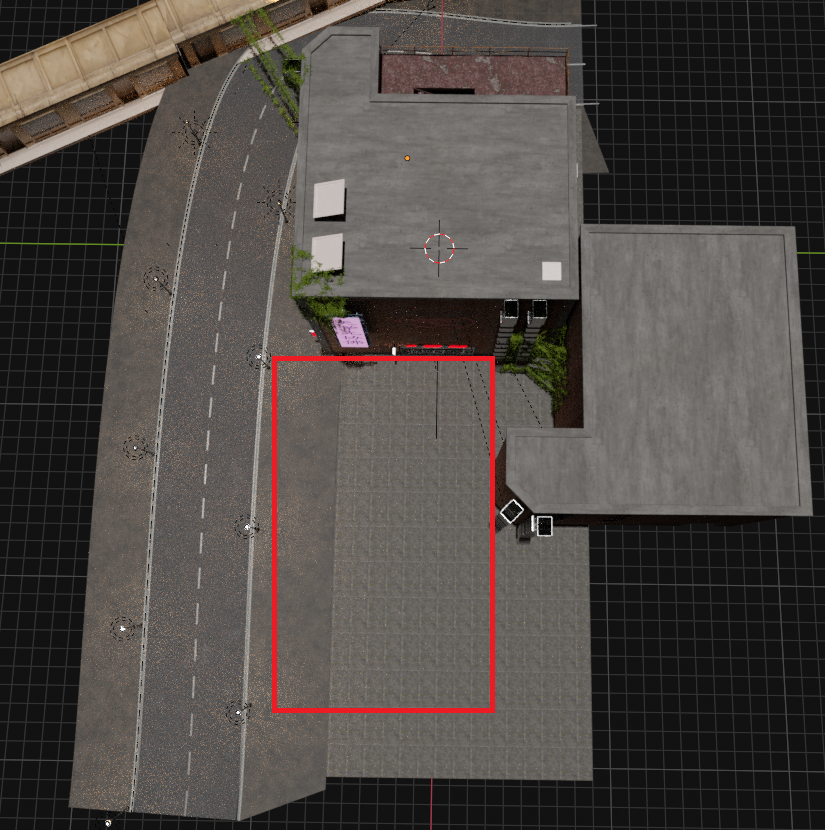
\includegraphics[width=1\columnwidth]{figures/defined_area.png}

    \caption{The defined area in the scene where we will acquire the data. The area is 20 x 13 meters and the z axis is kept constant at 1.7 meters. The images were captured every 0.5 meters.}
    \label{fig:defined_area}
\end{figure}

The area is along the x and y-axis, and the z-axis is kept constant. 
We programmed a Python script that captures the RGB and depth images of the scene at every 0.5 meters along the x and y-axis.
We used the equirectangular camera to capture images in 256x256 resolution, an example of the captured images at a certain point can be seen in figure \ref{fig:example_scene}. 
The total amount of taken images was 2268, half of them were RGB images and the other half were depth images. 
Next, we used the Delaunay triangulation to divide the scene into triangles and placed the probes at the vertices of the triangles, which can be seen on figure \ref{fig:delaunay}.
This way we have a uniform distribution of probes in the scene.

\begin{figure}[htb]
    \centering
    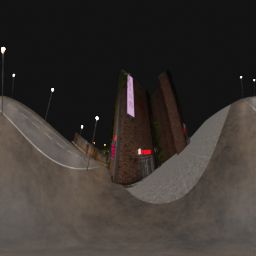
\includegraphics[width=0.49\columnwidth]{figures/camera_-13.0_8.0_1.7 image0001.png}
    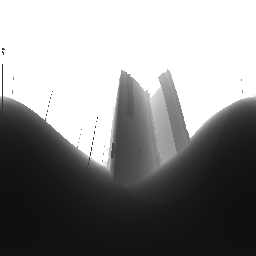
\includegraphics[width=0.49\columnwidth]{figures/camera_-13.0_8.0_1.7 depth0001.png}
    
    \caption{Example of the captured rgb and depth image at point (-13.0, 8.0, 1.7).}
    \label{fig:example_scene}
\end{figure}



\begin{figure}[htb]
    \centering
    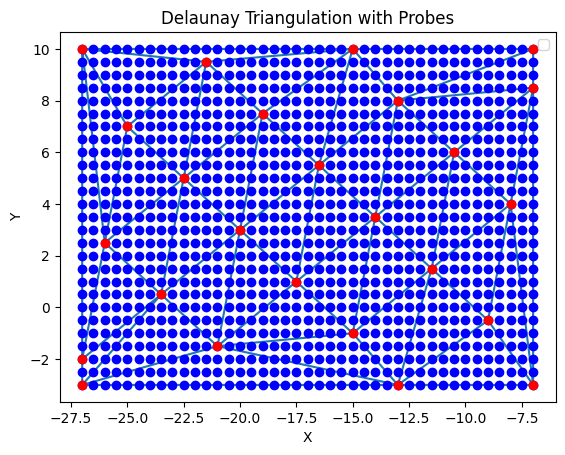
\includegraphics[width=\columnwidth]{figures/delaunay_triangulation.png}
    \caption{Delaunay triangulation of the scene. The probes that are marked with red are placed at the vertices of the triangles while the blue points are the points in the scene where we captured the data.}
    \label{fig:delaunay}
\end{figure}

\subsection{Interpolation with barycentric coordinates}
Interpolation with barycentric coordinates is basically a linear interpolation between the probes based on the barycentric coordinates of the point of interest in the triangle that the probes form and uses 3 points instead of 2 to interpolate the value at the point of interest.
The barycentric coordinates of a point in a triangle are the weights of the vertices of the triangle that sum up to 1.
The reflection at the point of interest is calculated as a weighted sum of the reflections of the probes (images taken at the vertices of the triangle).
The main advantage of this method is that it is simple and computationally efficient. However, it suffers from artefacts and inaccuracies since it only takes into account the weight of the probes with the probes themselves.
The results of the interpolation can be seen in figure \ref{fig:bilinear}. As expected, the reflections somewhat resemble the reflections in the scene, but they are not very accurate since the method just interpolates between the probes based on barycentric coordinates and does not take into account anything else.

\begin{figure}[htb]
    \centering
    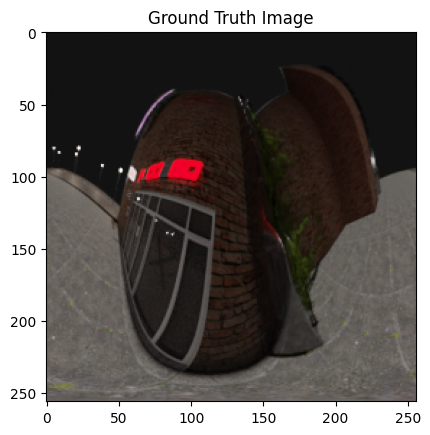
\includegraphics[width=0.49\columnwidth]{figures/ground_truth.png}
    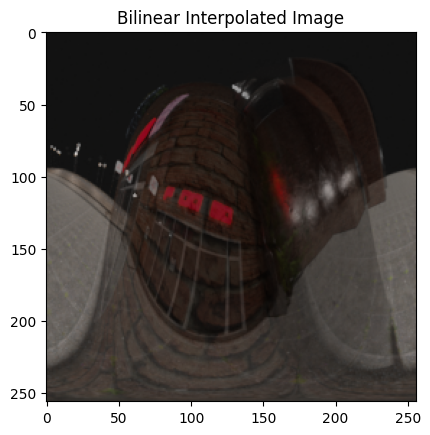
\includegraphics[width=0.49\columnwidth]{figures/bilinear.png}

    \caption{The results of the interpolation with barycentric weights. The left image is the ground truth reflection, the right image is the reflection calculated with interpolation.}
    \label{fig:bilinear}
\end{figure}

\subsection{Neural network approach}
Since the point of this seminar is to potentially improve the accuracy of the reflections calculated by simple methods such as interpolation with barycentric coordinates, we decided to implement a neural network that can predict the reflection at a given point in the scene based on the data from the probes.
The main part of the seminar was experimentation with different neural network architectures and training methods. 
We used TensorFlow library to implement the neural network in Python. Our first approach was to send each of the three probe RGB images for a given point through a convolutional neural network (CNN), then concatenate the outputs of the CNNs with the barycentric coordinates of the point and send the concatenated vector through a densely connected neural network layer. Finaly, we send this through convolutional layers and finally output the reflection at the point.
After a few experimentations and modifications of the network, we managed to get some results. The results of the first model can be seen in figure \ref{fig:neural_network_1}.
\begin{figure}[htb]
    \centering
    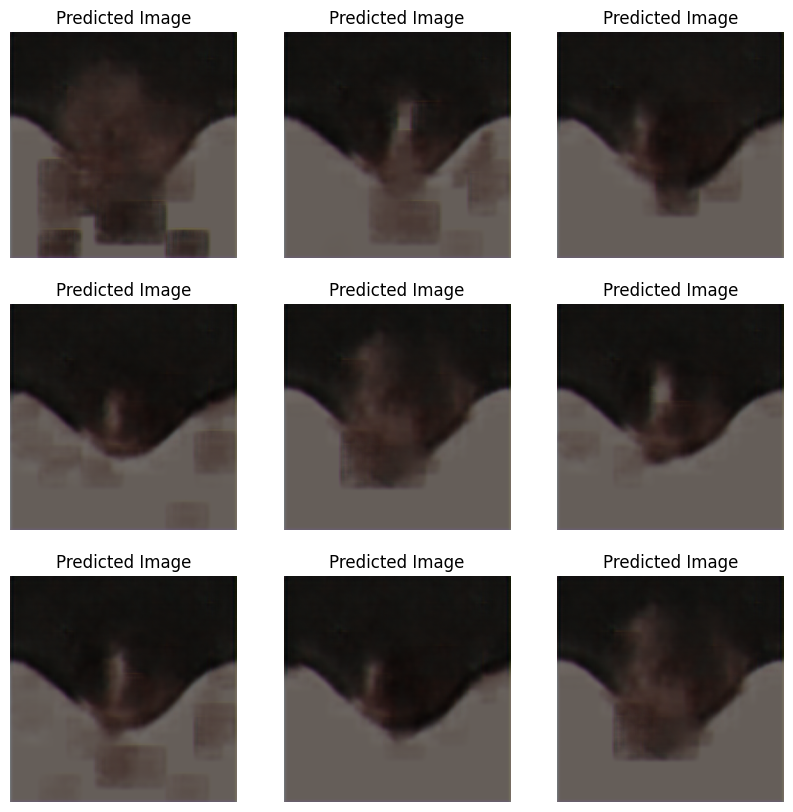
\includegraphics[width=0.49\columnwidth]{figures/experiment1_rgb_model.png}
    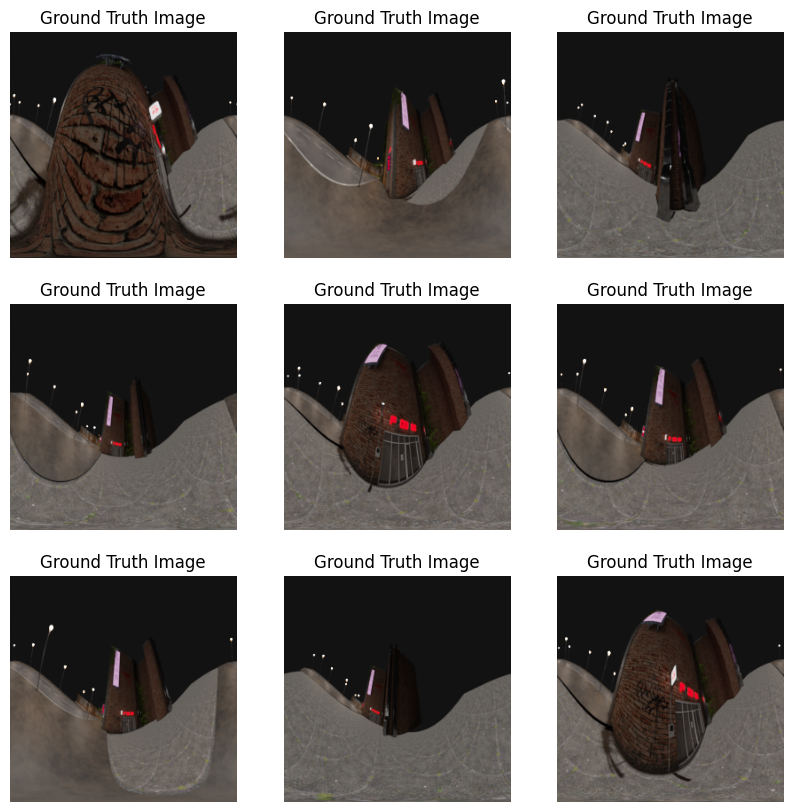
\includegraphics[width=0.49\columnwidth]{figures/experiment1_ground_truth.png}

    \caption{On the left image are model 1 predictions which takes into account RGB images and barycentric coordinates, on the right image is the ground truth.}
    \label{fig:neural_network_1}
\end{figure}
% TODO: comment on the results
We can see that the model managed to predict the general shapes and colors of objects in the scene, but the images are overall blurry.
The next step was to join the depth images of the probes into the network. We sent the depth images through the same CNN as the RGB images and concatenated the outputs with the RGB outputs and the barycentric coordinates.
The results of the second model can be seen in the figure \ref{fig:neural_network_2}. Surprisingly, the results were worse than the previous network that only used RGB images. In this case, the model only managed to predict the general shape of the floor, but the building is completely blended with the sky which is black in our scene.

\begin{figure}[htb]
    \centering
    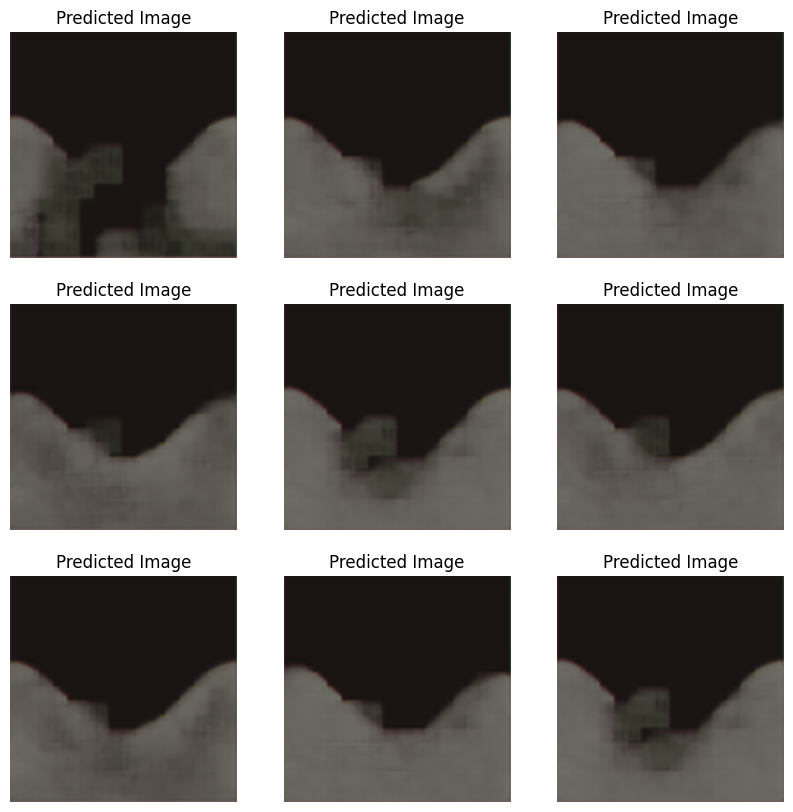
\includegraphics[width=0.49\columnwidth]{figures/experiment1_rgb_depth_model.png}
    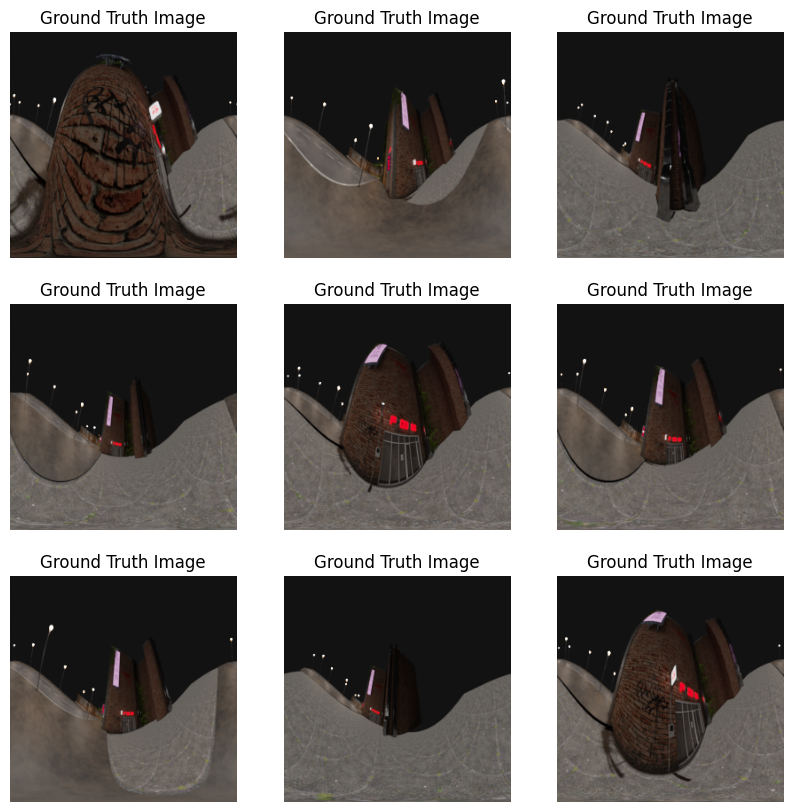
\includegraphics[width=0.49\columnwidth]{figures/experiment1_ground_truth.png}

    \caption{On the left image are model 2 predictions which takes into account RGB and depth images and barycentric coordinates, and on the right image is the ground truth.}
    \label{fig:neural_network_2}
\end{figure}

We tried to combat this by adding more convolutional layers and more neurons to the densely connected layer, but the results were still not satisfactory.
We also experimented with different loss functions such as Mean Squared Error (MSE), Structural Similarity Index (SSIM), Mean Absolute Error (MAE) and perceptual loss and found that MSE and MAE worked the best for our task.
Similarly, we experimented with different optimizers such as Adam, AdamW and SGD, and found that Adam and AdamW worked the best for our task, so we decided to experiment with combinations of these optimizers and loss functions.
The next experiment was to first concatenate the RGB and depth images of the probes and then send them through the CNN. The outputs of the CNN were then concatenated with the barycentric coordinates and sent through the densely connected layer.
The results were quite dissapointing, as the model was not able to predict any shapes or colors in the scene, the images was just a blurry mess.
The next step was to try a different architecture. We used similar convolutional layers as before, we only added batch normalization layers after each convolutional layer.
The major difference was that after we concatenated the outputs of the CNNs with the barycentric coordinates, we sent this through three densely connected layers starting with 1024 neurons and then halving the number of neurons in each layer.
We did this since having a high-dimensional initial layer ensures that the model has enough capacity to learn from the rich feature set generated by the CNN and the additional coordinates.
Halving of the number of neurons in subsequent layers helps in dimensionality reduction, leading to more abstract and general features. This process helps in better generalization by preventing the model from relying too heavily on potentially noisy or less important features.
We also added batch normalization and dropout layers after each densely connected layer. The results of this network can be seen in the figure \ref{fig:neural_network_3}.
As we can see the results are much better than the previous networks. The model managed to predict the general shapes and colors of the objects in the scene, but the images are still somewhat blurry.
\begin{figure}[htb]
    \centering
    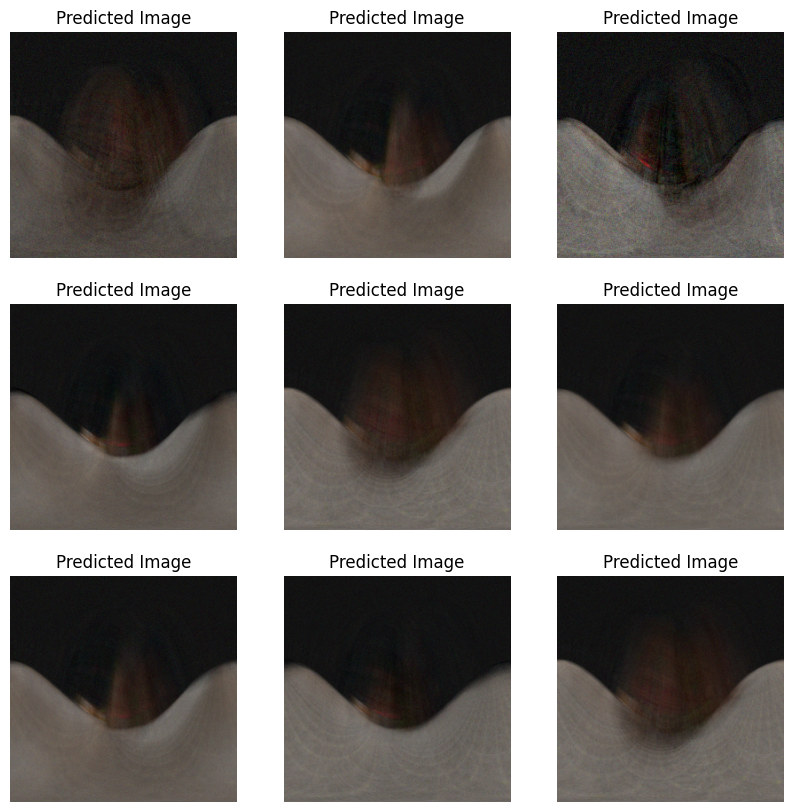
\includegraphics[width=0.49\columnwidth]{figures/experiment2_rgb_depth.png}
    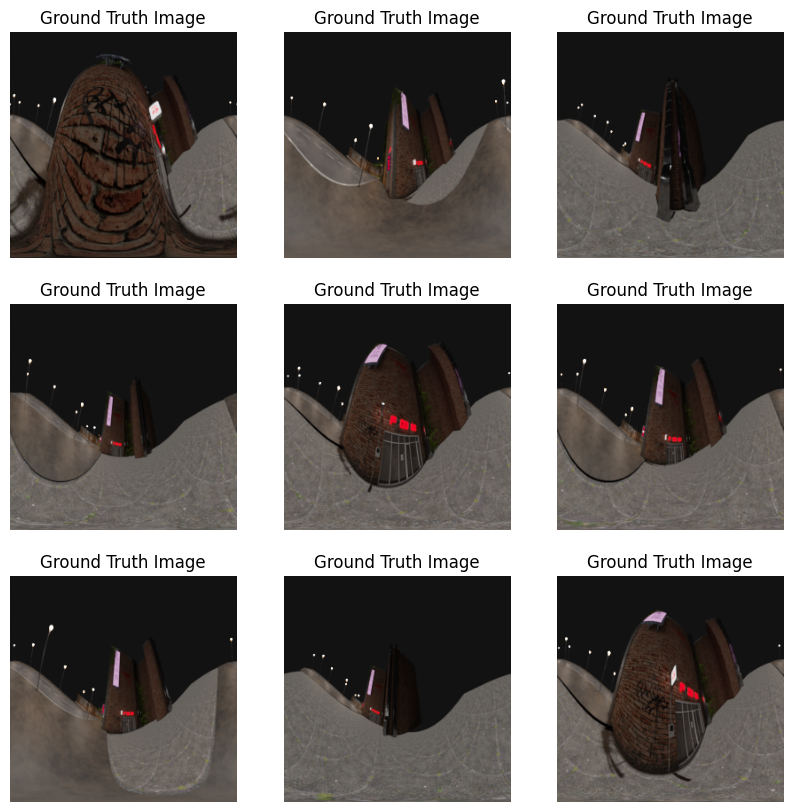
\includegraphics[width=0.49\columnwidth]{figures/experiment1_ground_truth.png}

    \caption{On the left image are the model 3 predictions which takes into account RGB and depth images and barycentric coordinates, on the right image is the ground truth.}
    \label{fig:neural_network_3}
\end{figure}

We tried to improve the performance of the network by adding positional encoding to the input images. Theoretically, this should help the network to better understand the spatial relationships between the probes and the point of interest.
The results of this network can be seen in the figure \ref{fig:neural_network_4}. The results are more blurry than the previous network, but the vivid colors are more accurate.

\begin{figure}[htb]
    \centering
    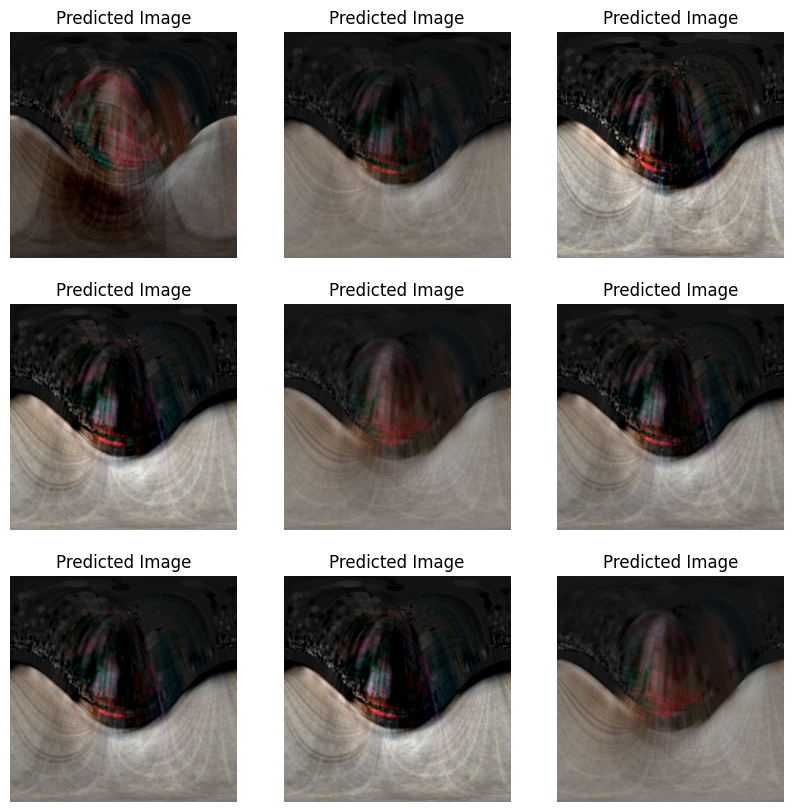
\includegraphics[width=0.49\columnwidth]{figures/experiment3_positional_encoding_rgb_depth.png}
    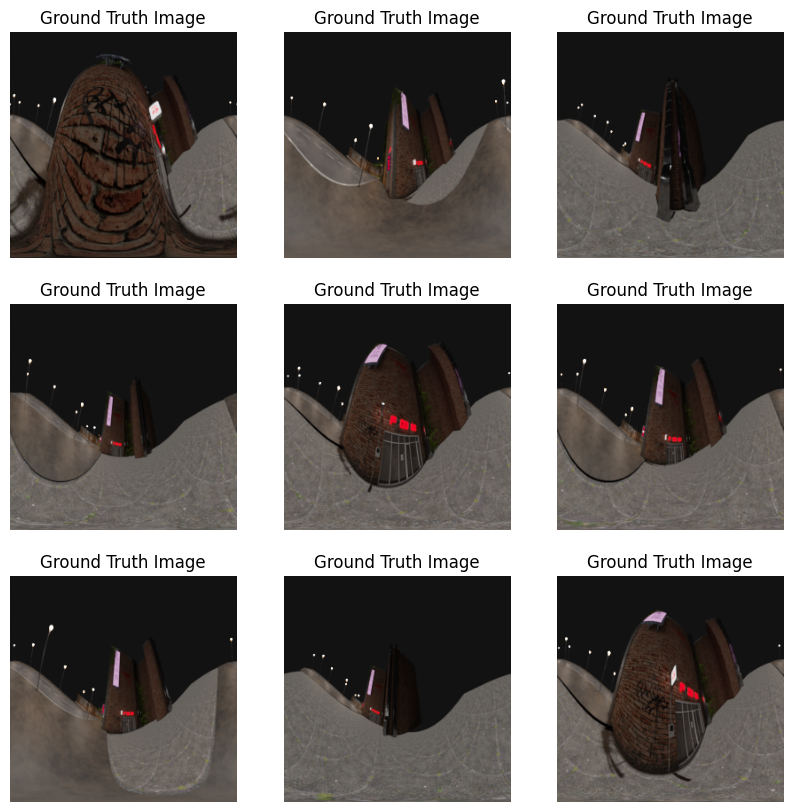
\includegraphics[width=0.49\columnwidth]{figures/experiment1_ground_truth.png}

    \caption{On the left image are model 4 predictions which takes into account positionally encoded RGB and depth images, barycentric coordinates, on the right image is the ground truth.}
    \label{fig:neural_network_4}
\end{figure}


\section{Results}

For the evaluation of the results we decided to use the LPIPS (Learned Perceptual Image Patch Similarity) metric, which is a perceptual similarity metric that is trained with a dataset of human perceptual similarity judgments and more appropriately reflects the human
perception preferences than the VGG perceptual loss~\cite{jo2020investigating}. The metric is designed to measure the perceptual similarity between two images.
We used the LPIPS metric to compare the predicted reflections of the neural network to the ground truth reflections (the lower the better).
During the extensive experimentation with different architectures, loss functions and optimizers, we were saving the best models and were planning on evaluating them in the end.
The problem occurred when we tried to load the models that we saved. We discovered that Keras does not directly support one of the operations in our model and the models could not be loaded correctly.
It turns out that operation \(conv\_output = input\_images[:, i, :, :, :]\) involves slicing a tensor, which is a common operation in NumPy but is not directly supported in Keras layers. The main reason Keras doesn't directly support such an operation is that Keras models are designed to be symbolic and fully differentiable, meaning every operation in the model must be a Keras/TensorFlow operation that supports backpropagation.
To perform slicing within a Keras model, you need to define a custom layer that performs the slicing operation using TensorFlow operations.
We did not have enough time to relearn the models and evaluate them, since it took a long time to train the models (we don't have access to a GPU) and they are not directly relearnable due to the usage of random dropout layers.
We decided to evaluate the performance on a simplified model that we could relearn in a reasonable amount of time. The model was the adjusted model 3 that initially used both RGB and depth images and barycentric coordinates, but we removed the depth images from the input so that we only used RGB images and reduced the number of epochs to 12.
The loss curve of training the simplified model can be seen in the figure \ref{fig:loss_curve}.
\begin{figure}[htb]
    \centering
    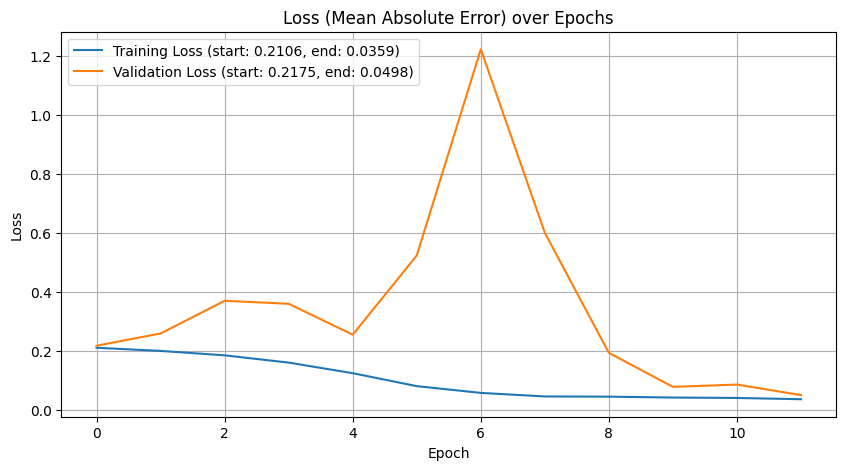
\includegraphics[width=\columnwidth]{figures/loss_curve.png}

    \caption{The loss curve (Mean Absolute Error) of the simplified model 3 using only RGB images and barycentric coordinates.}
    \label{fig:loss_curve}
\end{figure}

The loss curve shows that the model was learning well and that both the training and validation loss were decreasing, even though the validation loss was slightly higher than the training loss and had some fluctuations.
Evaluation of the model on the test set with the LPIPS metric can be seen in the table \ref{table:lpips_bilinear}. 
The results are the average LPIPS score of the predictions of the model on the test set.

\begin{table}[htb]
    \centering
    \begin{tabular}{|c|c|} \hline
    Model & LPIPS \\ \hline
    Barycentric interpolation & 0.28 \\ \hline
    Simplified model 3 & 0.51 \\ \hline
    \end{tabular}
    \caption{The LPIPS score of the barycentric interpolation and the simplified model 3.}
    \label{table:lpips_bilinear}
\end{table}

As we can see, the model achieved an LPIPS score of \textbf{0.51} which is not the best since we achieved better results with the barycentric weight interpolation method.
We would probably achieved better results if we could evaluate the best models that we saved during the experimentation (that also used depth images), but we assume that the LPIPS score would still be higher than the barycentric weight interpolation method.
Overall, the trained model did a good job at predicting the general shapes and colors of the objects in the scene, but the images are still blurry and the changes in the position of the objects are not very well captured since it tries to generalize the reflections in the scene in a way that the loss is overall minimized. The problem with generating accurate images at the different points in the scene can be seen in the simulated circle movement of the camera in the scene, which can be seen in gif at~\cite{gif}.
We assume that we could achieve better results if we experimented with a scene where the sky is not visible or is not black, since the images in our dataset mostly had at least a third of the image black, which the model predicted easily and was given a false sense of accuracy. 

\section{Conclusion}

In conclusion, in this seminar, we investigated interpolation methods for improving real-time reflective material rendering using reflection probes. 
We compared interpolation with barycentric weights with neural network-based approaches to enhance reflection accuracy.
Our experiments began with basic barycentric interpolation, revealing limitations in capturing accurate reflections.
We then developed and tested several neural network models, incorporating RGB and depth images along with barycentric coordinates. 
The most effective model utilized a combination of convolutional and densely connected layers, but the results were not as accurate as the barycentric interpolation method.
We believe that the approach we choose is not suitable for our task, since the neural networks are generally slow and in our case not performing better than the simple interpolation method.
We believe that we could achieve better results with a different approach, such as using a generative adversarial network (GAN), a larger dataset and include also the normal maps of the scene in the input.


%\bibliographystyle{eg-alpha}
\bibliographystyle{eg-alpha-doi}

\bibliography{egbibsample}

%-------------------------------------------------------------------------
\newpage




\end{document}
 